\documentclass{article}
\usepackage[T1]{fontenc}

\usepackage{graphicx}
\usepackage{listings}
\begin{document}

\title{FOSS Lab Report}
\author{Gokul K\\[2\baselineskip]
Roll Number: 21\\[2\baselineskip]}
\date{20 January 2020}

\maketitle

\section{Advanced Linux Commands}
\subsection{Aim}
To familiarise advanced linux commands
\subsection{Commands}
\subsubsection{cURL}
cURL stands for client URL. curl is a tool to transfer data from or to a server, using one of the supported protocols (DICT, FILE, FTP, FTPS, GOPHER, HTTP, HTTPS, IMAP, IMAPS, LDAP, LDAPS, POP3, POP3S, RTMP, RTSP, SCP, SFTP, SMB, SMBS, SMTP, SMTPS,
TELNET and TFTP). The command is designed to work without user interaction.\newline\newline
\hspace{\parindent} {\em usage}: curl [options] location
\newline
\hspace{\parindent} {\em options}:\newline
\begin{itemize}
    \item -H: to add headers to the request
    \item -d: to specify data, can be used with X
    \item -X: to specify method
    \item -v: to get verbose response
    
\end{itemize}
    
\begin{figure}
    \centering
    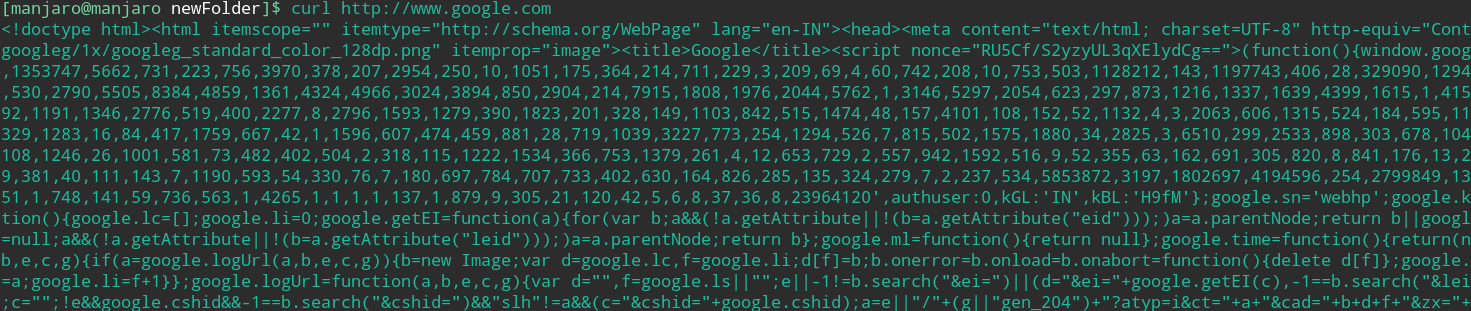
\includegraphics[width=.80\textwidth]{img/p3/ss1.png}
    \caption{Sample input/output of curl commands}
\end{figure}

\subsubsection{ssh}
ssh (SSH client) is a program for logging into a remote machine and for executing commands on a remote machine. It is intended to replace rlogin and rsh, and provide secure encrypted communications between two untrusted hosts over an insecure network. X11 connections and arbitrary TCP/IP ports can also be forwarded over the secure channel.
\begin{enumerate}
    \item {\bf ssh}: Used to logging into a remote server\newline
    \hspace{\parindent} {\em usage}: ssh [username@]hostname \newline
    
    \item {\bf scp}: Used to copy file from/into a remote server\newline
    \hspace{\parindent} {\em usage}: scp [username@]sourcehost:location [username@]desthost:location\newline
    
\end{enumerate}
\subsubsection{wget}
GNU wget is a free utility for non-interactive download of files from the Web.It supports
HTTP , HTTPS , and FTP protocols, as well as retrieval through HTTP proxies.
Wget is non-interactive, meaning that it can work in the background, while the user
is not logged on. This allows you to start a retrieval and disconnect from the system,
letting Wget finish the work. By contrast, most of the Web browsers require constant
user’s presence, which can be a great hindrance when transferring a lot of data.

\begin{figure}[h!]
    \centering
    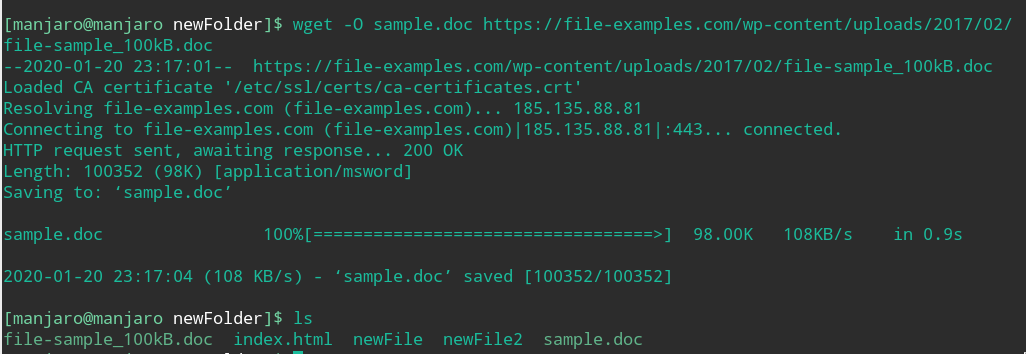
\includegraphics[width=.80\textwidth, width=.83\textwidth]{img/p3/ss2.png}
    \caption{Sample input/output of wget command}
\end{figure}

\subsubsection{ftp}
The FTP (File Transfer Protocol) utility program is commonly used for copying files
to and from other computers. These computers may be at the same site or at different
sites thousands of miles apart. FTP is a general protocol that works on UNIX systems
as well as a variety of other (non-UNIX) systems. To connect your local machine to the remote machine, type
\begin{verbatim}
    ftp machinename
\end{verbatim}

\subsubsection{grep}
grep is a command-line utility for searching plain-text data sets for lines that match a regular expression. Its name comes from the ed command g/re/p, which has the same effect: doing a global search with the regular expression and printing all matching lines.
\begin{figure}[h!]
    \centering
    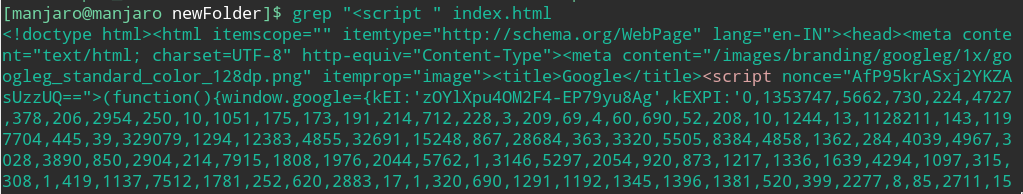
\includegraphics[width=.83\textwidth]{img/p3/ss3.png}
    \caption{Sample input/output of grep command}
\end{figure}

\subsection{Result}
The above commands are executed and output is verified
\end{document}